This appendix provides various additional figures and tables to complete the analysis.

\subsubsection{Occupational outcomes at age 42}

This subsection provides additional results concerning the outcomes for individuals at age 42. We first provide an alternative depiction of the results provided in Figure \ref{chap2-fig:occ-multi2-pinc} to further illustrate the relationship between parental income and occupational dynamics. Figure \ref{chap2-fig:occ-multi2-quant-male} reports the \emph{change} across the two cohorts in the probability of being in each occupational category at age 42. For each decile in the parental-income distribution, we report the probabilities of being in each of the four occupations, when using the estimates in Table \ref{chap2-tab:occ-multi2-short}. The figure hence indicates how the probability of being in, say, a high-paying occupation for the cohort born in 1970 has changed for a particular parental-income decile relative to what that probability was for those born in 1958. 

\begin{figure}[!tb]
    \centering
    \caption{Change across cohorts in the probability of being in each occupation at age 42 (in percentage points)}
    \label{chap2-fig:occ-multi2-quant-male}
    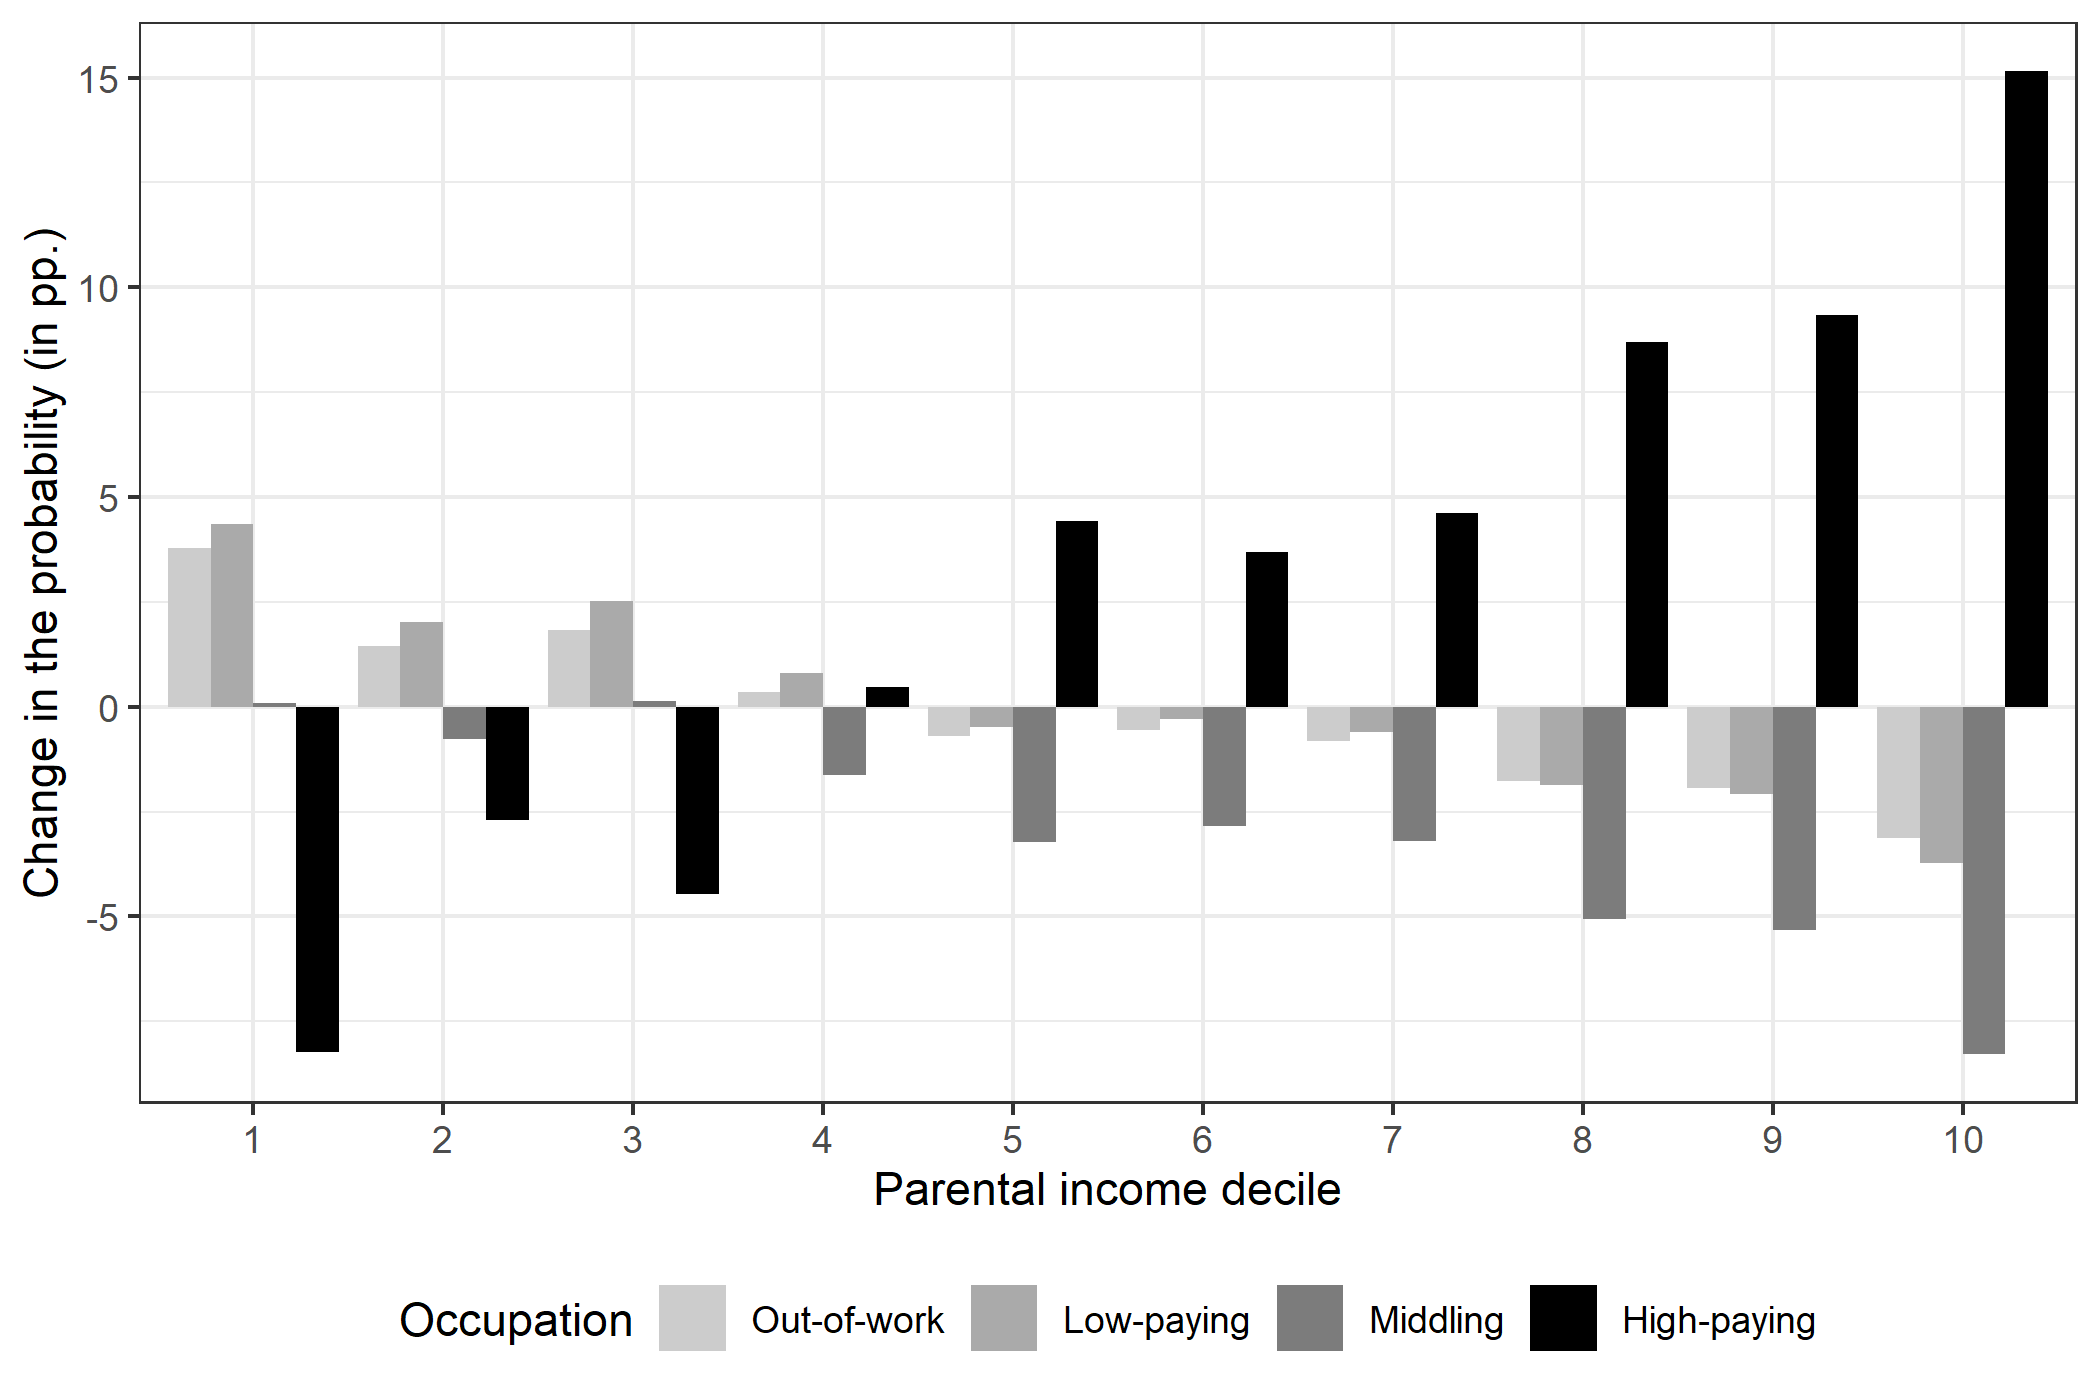
\includegraphics[width=\linewidth]{chap2/graphic/occ-multi2-quant-male.png}
 	\vspace{-3em}
 	\justify\singlespacing\footnotesize{\textit{Notes:} This figure shows the difference, expressed in percentage points, between the BCS70 and NCDS58 cohorts in terms of probability of being in each type of occupation (out-of-work, low-paying, middling, high-paying) at age 42 according to the decile of the parental income distribution. 
 	Probabilities are computed for males in both cohorts at each parental income decile, according to the multinomial logistic regression reported in columns (1) of Table \ref{chap2-tab:occ-multi23-base}.}
 \end{figure}
 
Not surprisingly, for almost all parental-income categories the likelihood of being in a middling job has declined for the younger cohort. The exception are those in the first and third deciles, for whom there has been a small increase. Yet, whether this decline is offset by an increase in the probability of working in a low- or a high-paying occupation is strongly dependent on parental income. It is only for those in the fourth decile that we see the pattern observed in the aggregate data: a reduction in the share of middling jobs accompanied by an increase in that of both low- and high-paying ones. Everywhere else in the distribution the changes in the share of high- and low-paying occupations are of opposite sign. For those in the top half of the parental-income distribution, the decline in the share of middling occupations has been accompanied by lower shares of individuals in both low-paying jobs and out of work and a higher share in high-paying occupations. The magnitude of these changes increases with parental income. For those in the top decile, the proportion of individuals in high-paying jobs rose by 15.1 pp., while that of those in middling fell by 8.3 pp. The bottom three deciles display an increase for out-of-work and low-paying and a decline for high-paying, irrespective of whether there was a positive or negative change in the share of middling jobs, though the magnitudes for the latter are small an all three cases.

Figure \ref{chap2-fig:occ-multi3-pinc-female} provides the change in the probability of being in each occupation in the second period conditional on first-period occupation at several points of the parental income distribution for females. 

\begin{figure}[!htb]
    \centering
    \caption{Change in probability to be in each occupation in the second period according to the first-period occupation and parental income (female only)}
    \label{chap2-fig:occ-multi3-pinc-female}
    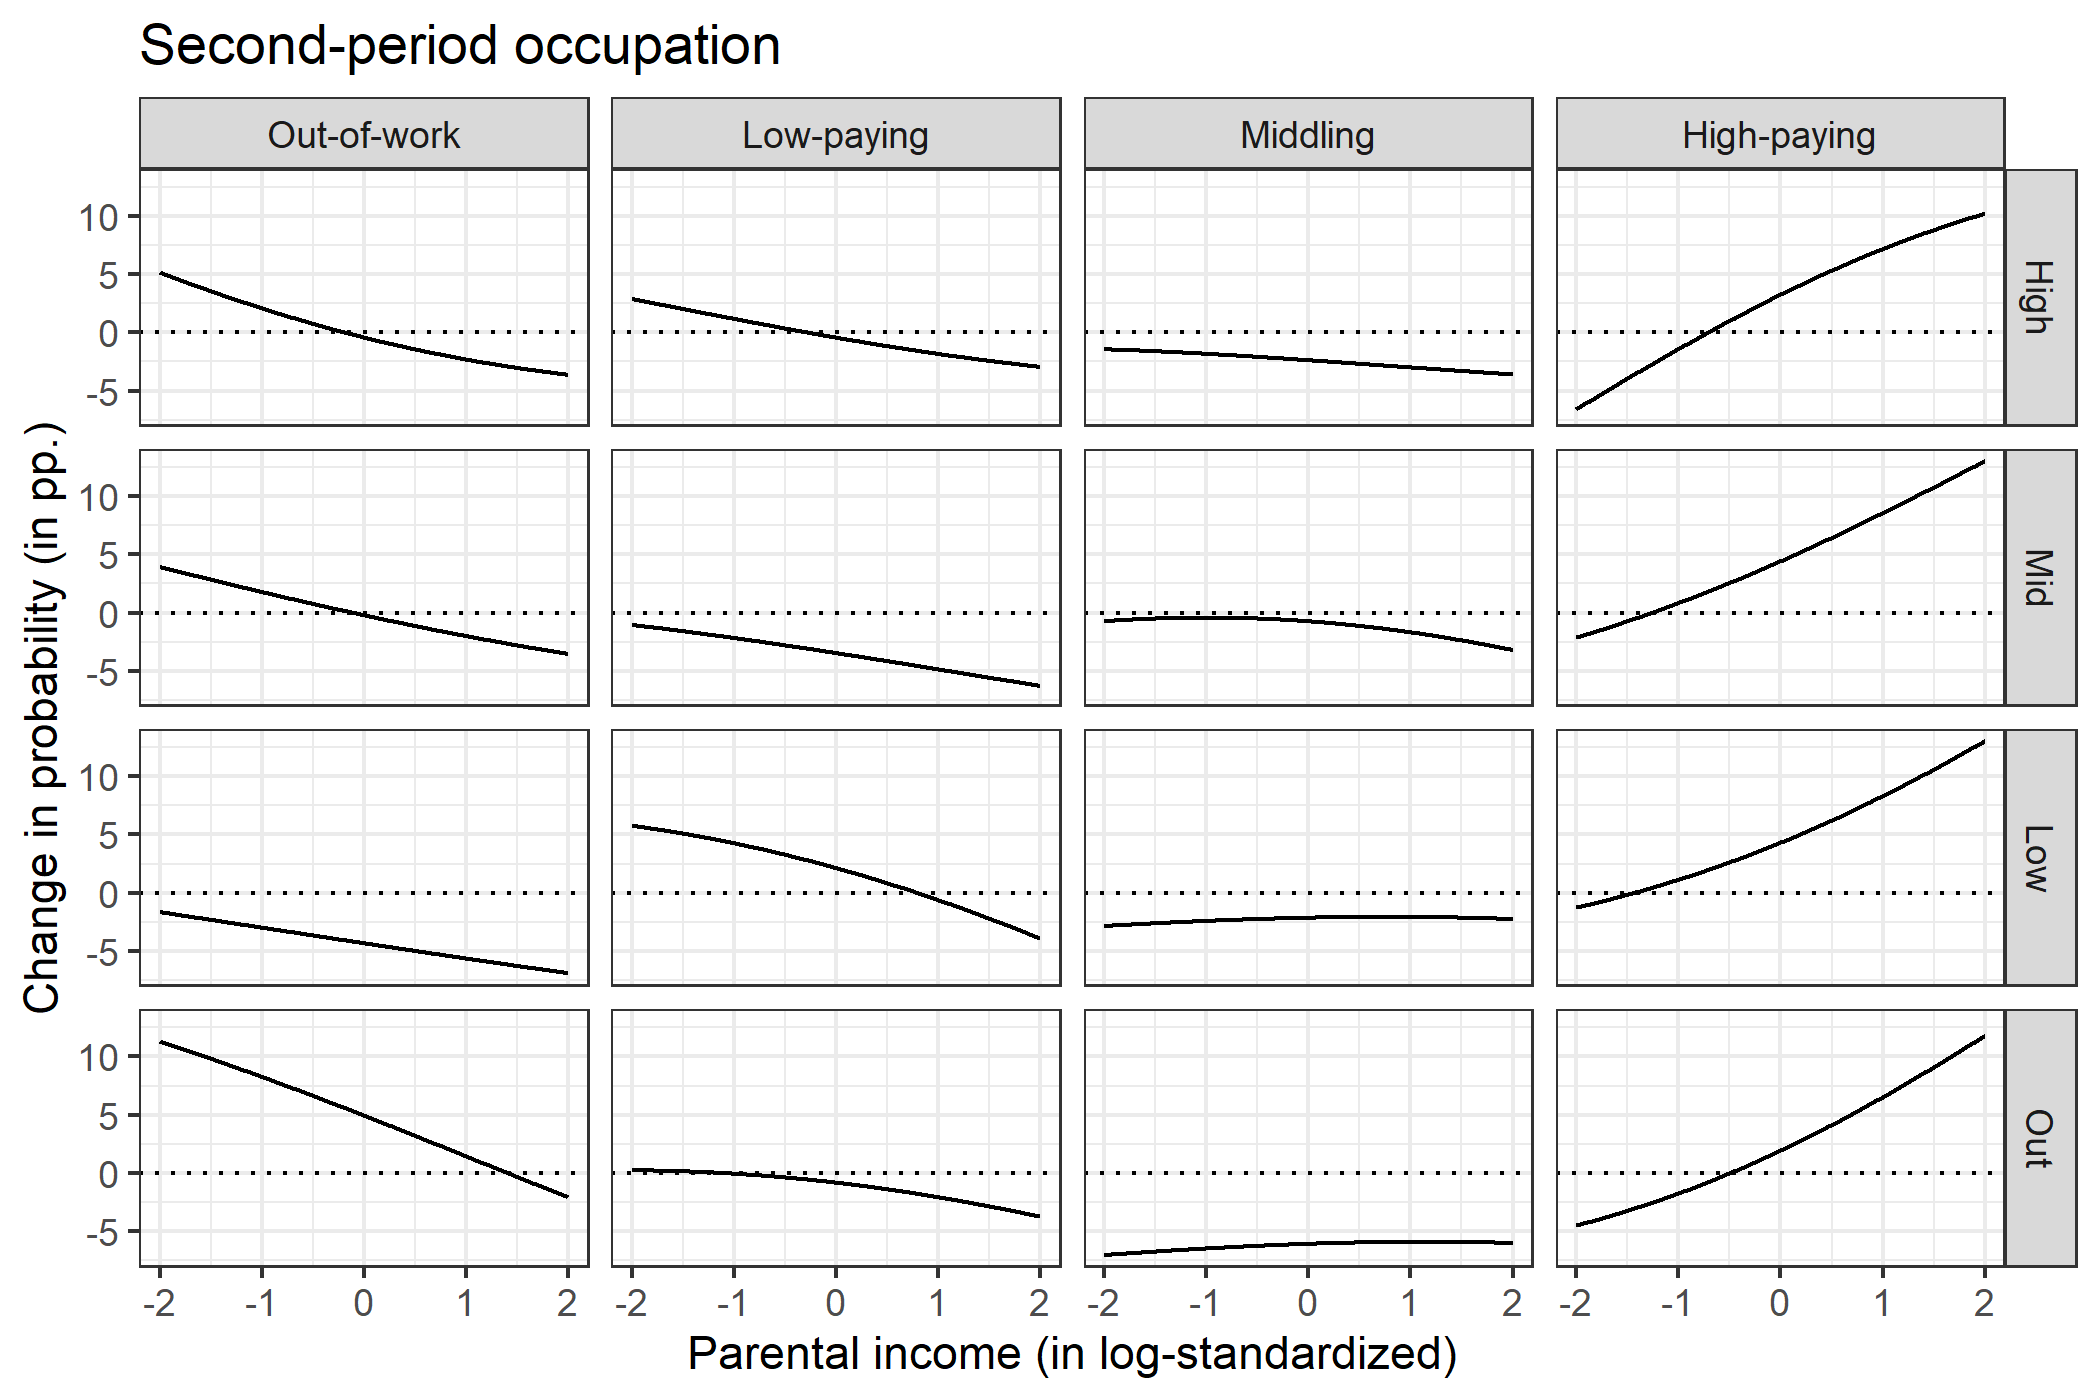
\includegraphics[width=\linewidth]{chap2/graphic/occ-multi3-pinc-female.png}
    \vspace{-3em}
    \justify\singlespacing\footnotesize{\textit{Notes:} This figure presents the difference, expressed in percentage points, between the BCS70 and the NCDS58 cohorts in terms of probability of being in each type of second-period occupation (out-of-work, low-paying, middling, high-paying), conditional on the first-period occupation, according to parental income, in log-standardized.
    Probabilities are computed for females in both cohorts according to the multinomial logistic regression reported in columns (2) of Table \ref{chap2-tab:occ-multi23-base}.}
\end{figure}

We summarize the results on transition probabilities in Table \ref{chap2-tab:mob-pinc-both}. The table reports changes in the probability of each type of mobility depending on the individual’s initial occupation, assessed at several points of the parental income distribution as in the graphs above. The left panel of the table provides the results for men, the right panel for women.
\begin{table}[!tb]
    \centering
    \caption{Change in intra-generational mobility across cohorts}
    \label{chap2-tab:mob-pinc-both}
    \begin{threeparttable}
        \setlength{\tabcolsep}{9pt}
        
\begin{tabular}{lrrrrrr}
\toprule
\multicolumn{1}{c}{} & \multicolumn{3}{c}{Male} & \multicolumn{3}{c}{Female} \\
\cmidrule(l{3pt}r{3pt}){2-4} \cmidrule(l{3pt}r{3pt}){5-7}
First-period occupation & Down & Persist & Up & Down & Persist & Up\\
\midrule
& \multicolumn{3}{c}{\textit{at +2 STD}} & \multicolumn{3}{c}{\textit{at +2 STD}}\\ 
\midrule
Out-of-work &  & -0.57 & 0.57 &  & -2.05 & 2.05\\
Low-paying & -4.41 & -0.88 & 5.29 & -6.88 & -3.90 & 10.78\\
Middling & -3.84 & -0.52 & 4.36 & -9.82 & -3.20 & 13.02\\
High-paying & -2.95 & 2.95 &  & -10.19 & 10.19 & \\
\midrule 
 & \multicolumn{3}{c}{\textit{at the Mean}} & \multicolumn{3}{c}{\textit{at the Mean}}\\ 
\midrule
Out-of-work &  & 4.92 & -4.92 &  & 4.96 & -4.96\\
Low-paying & -2.70 & 4.83 & -2.13 & -4.32 & 2.14 & 2.18\\
Middling & -0.70 & 3.65 & -2.95 & -3.68 & -0.74 & 4.42\\
High-paying & 2.54 & -2.54 &  & -3.25 & 3.25 & \\
\midrule 
 & \multicolumn{3}{c}{\textit{at -2 STD}} & \multicolumn{3}{c}{\textit{at -2 STD}}\\ 
\midrule
Out-of-work &  & 11.27 & -11.27 &  & 11.30 & -11.30\\
Low-paying & -0.53 & 9.57 & -9.04 & -1.65 & 5.76 & -4.11\\
Middling & 3.29 & 5.41 & -8.70 & 2.87 & -0.74 & -2.14\\
High-paying & 10.92 & -10.92 &  & 6.58 & -6.58 & \\
\bottomrule
\end{tabular}

            \begin{tablenotes}[flushleft]
                \footnotesize{\item \textit{Notes}: This Table summarizes the difference, expressed in percentage points, between the BCS70 and the NCDS58 cohorts in terms of type of mobility (down, persist, up) conditional on first period occupation (out-of-work, low-paying, middling, high-paying) at several points of the parental income distribution (at +2 std., at the mean, at -2 std.). These values are computed from the results obtained in Figure \ref{chap2-fig:occ-multi3-pinc-male} for males and in Figure \ref{chap2-fig:occ-multi3-pinc-female} for females.}
            \end{tablenotes}
    \end{threeparttable}
\end{table}

\subsubsection{Results at the regional level}\label{chap2-app-additional-regional}

Figures \ref{chap2-fig:reg-multi2-pinc-male} and \ref{chap2-fig:reg-multi2-pinc-female} depict the probabilities of being in each second period occupation according to parental income at the regional level, for men and women respectively. Figure  \ref{chap2-fig:regocc-absolute-all} depicts the correlation between the change in the parental income coefficient for second-period occupations and the change in job polarization at the regional level.

\begin{figure}[!htb]
    \centering
    \caption{Second-period occupation probability according to parental income at the regional level (male only)}
    \label{chap2-fig:reg-multi2-pinc-male}
    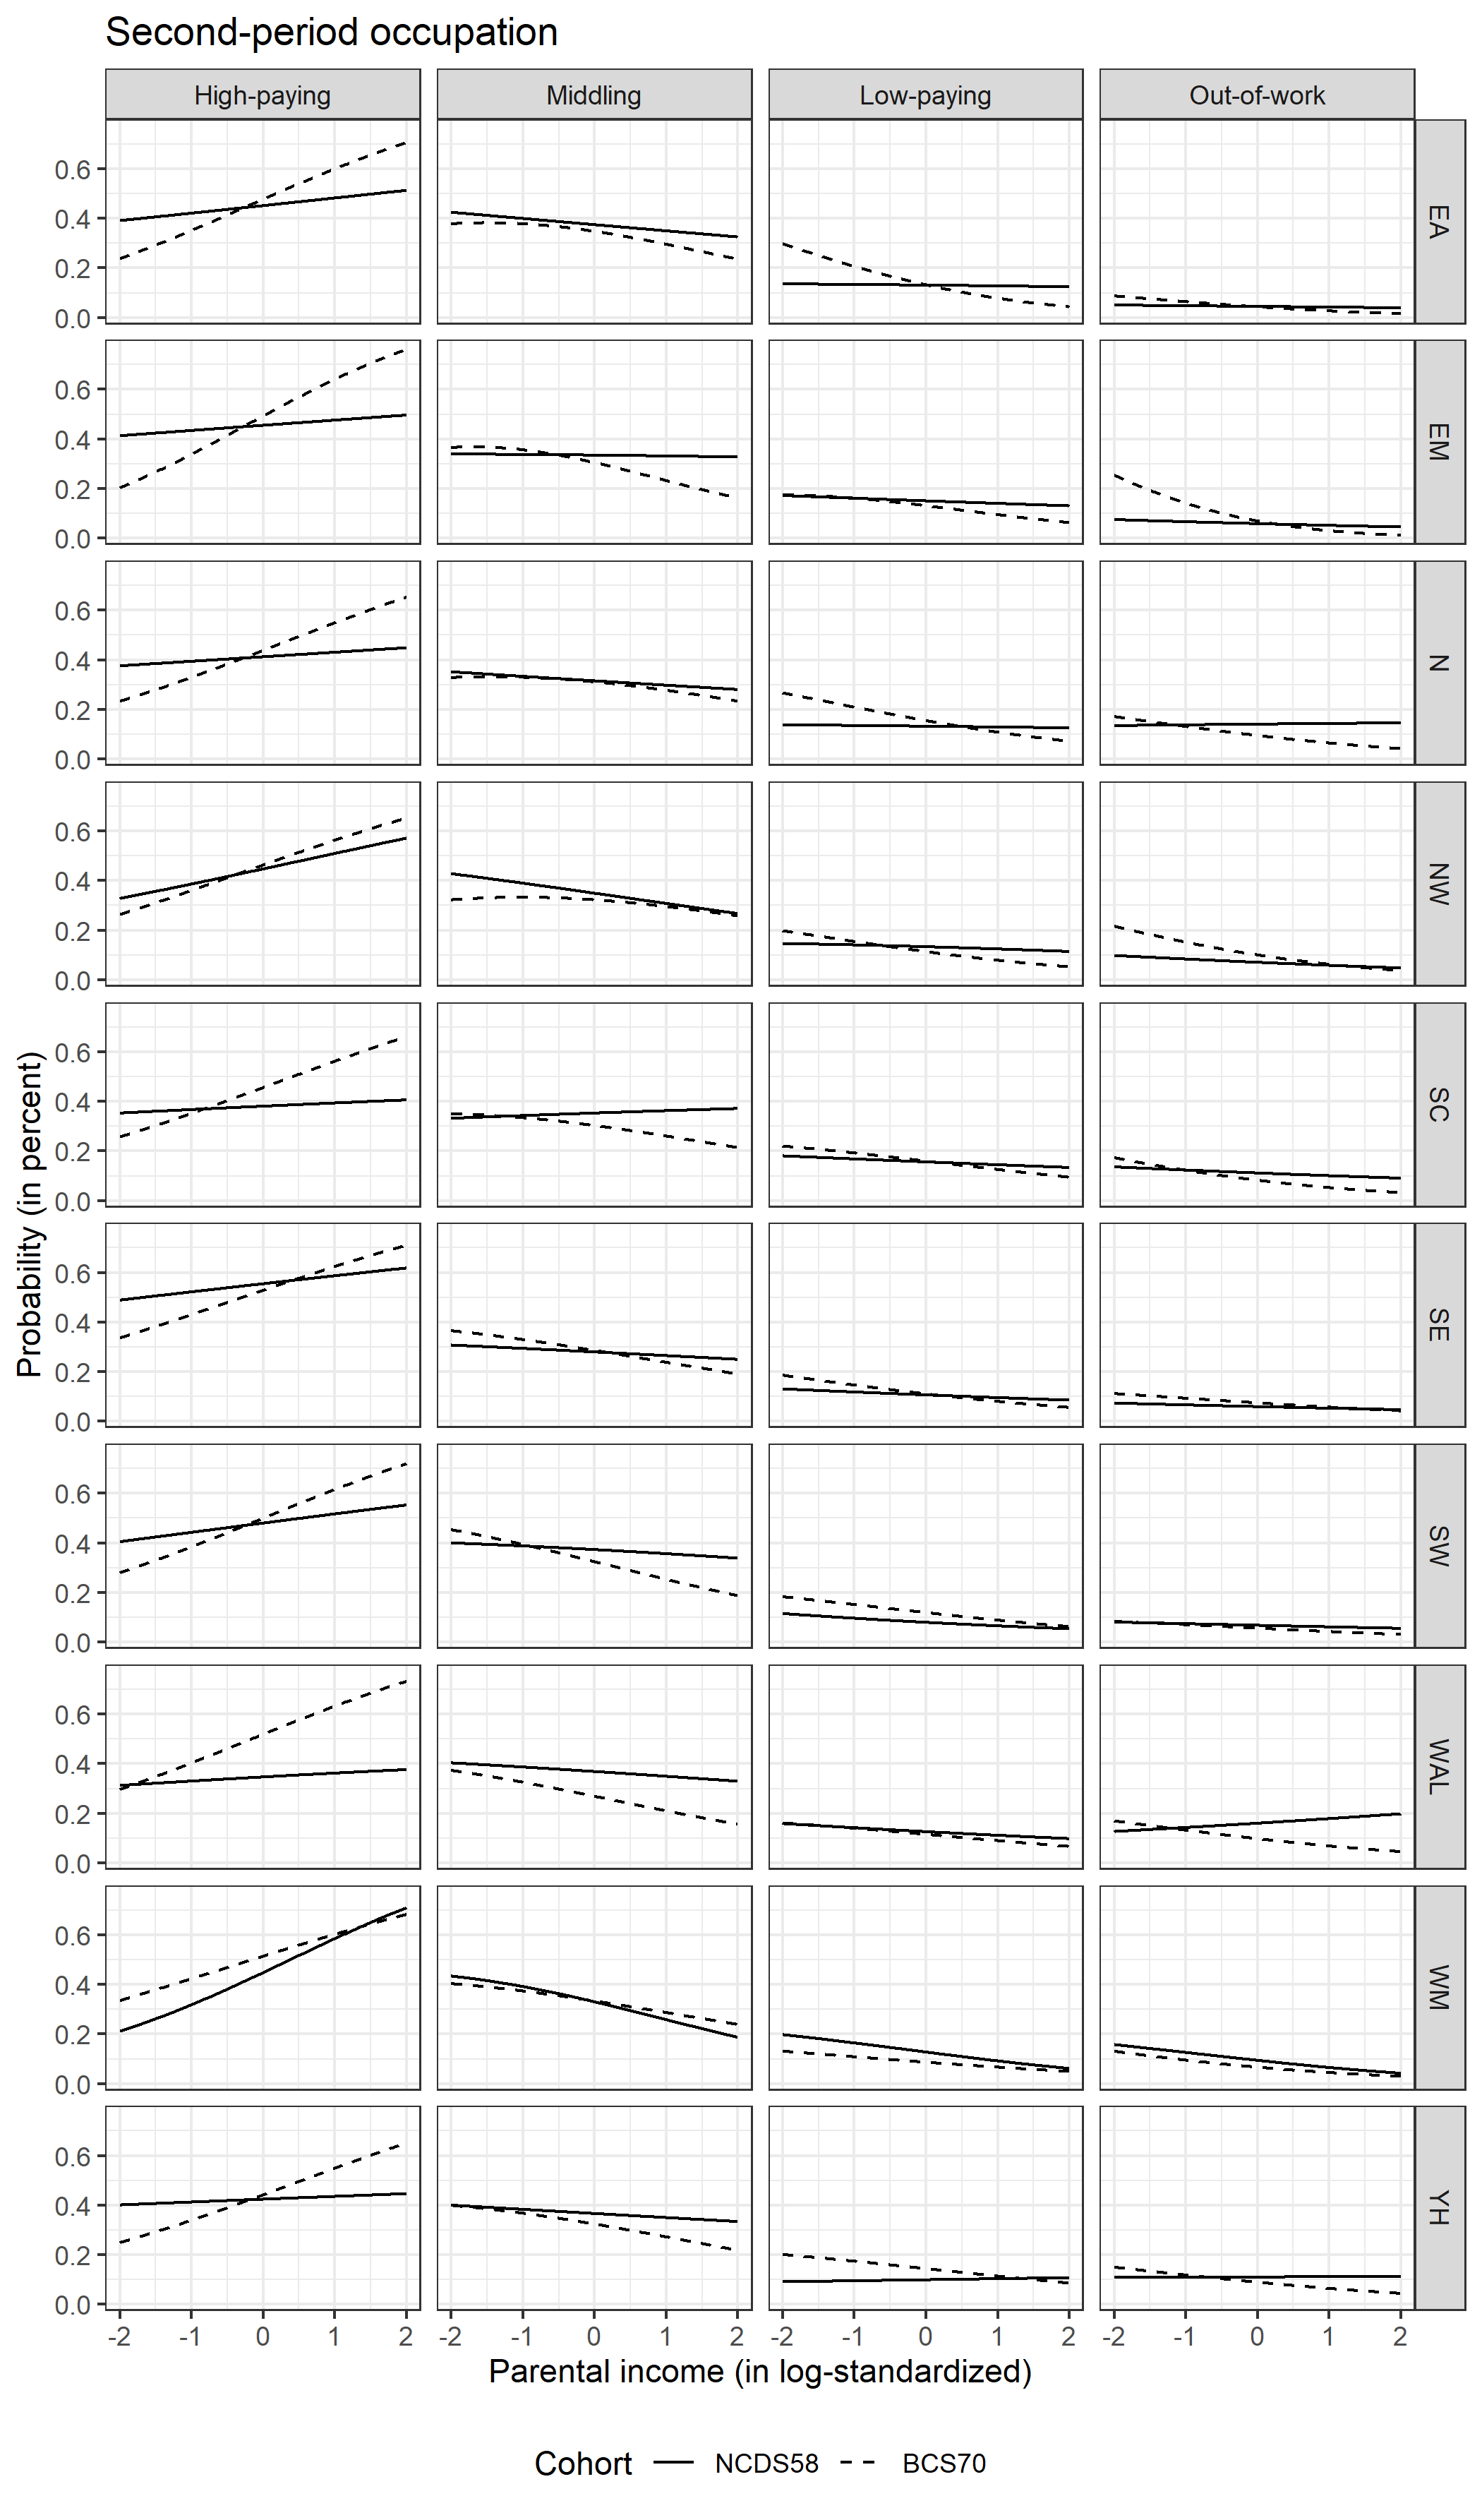
\includegraphics[width=.7\linewidth]{chap2/graphic/reg-multi2-pinc-male.png}
    \vspace{-3em}
	\justify\singlespacing\footnotesize{\textit{Notes:} This figure presents the probability, expressed in percent, of being in each type of occupation (out-of-work, low-paying, middling, high-paying) in second period according to parental income, in log-standardized, for each region.
	Probabilities are computed for males in both cohorts according to the multinomial logistic regressions reported in Table \ref{chap2-tab:reg-multi2-short}.}
\end{figure}

\begin{figure}[!htb]
    \centering
    \caption{Second-period occupation probability according to parental income at the regional level (female only)}
    \label{chap2-fig:reg-multi2-pinc-female}
    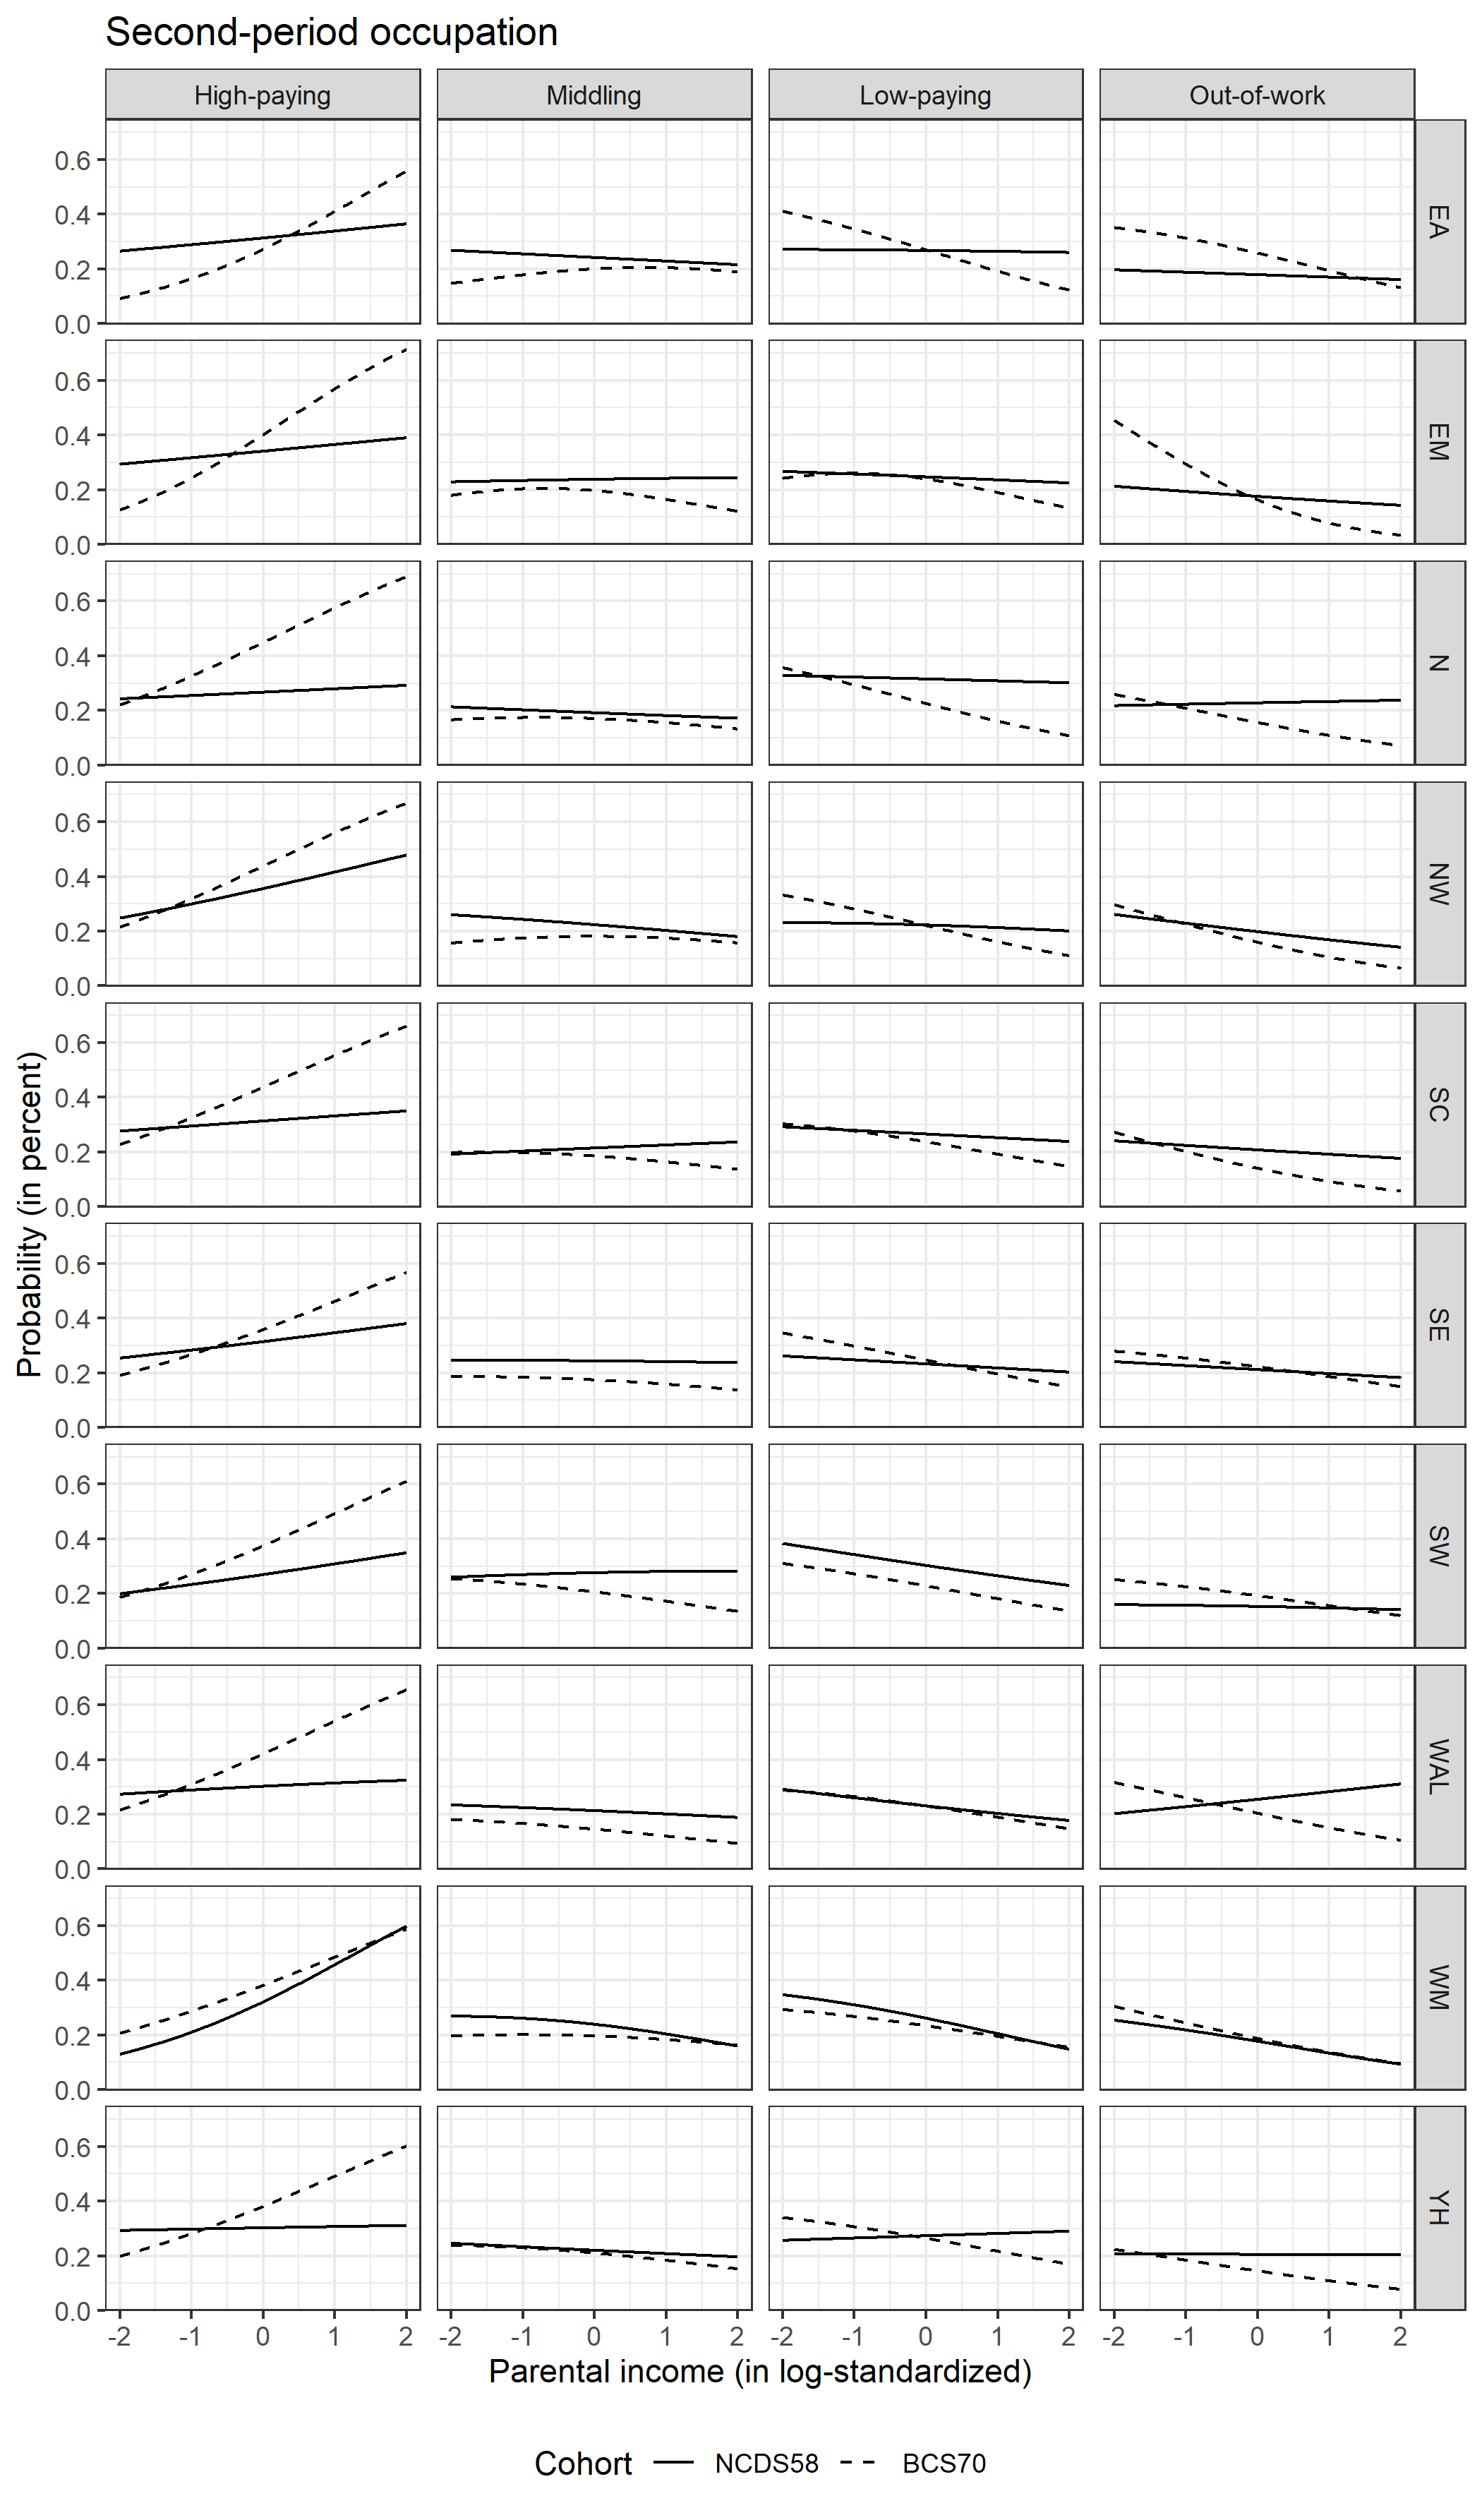
\includegraphics[width=.7\linewidth]{chap2/graphic/reg-multi2-pinc-female.png}
    \vspace{-3em}
	\justify\singlespacing\footnotesize{\textit{Notes:} This figure presents the probability, expressed in percent, of being in each type of occupation (out-of-work, low-paying, middling, high-paying) in second period according to parental income, in log-standardized, for each region.
	Probabilities are computed for females in both cohorts according to the multinomial logistic regressions reported in Table \ref{chap2-tab:reg-multi2-short}.}
\end{figure}

\begin{landscape}
\begin{table}[!tb]
    \centering
    \caption{Probability of being in each occupation in the second period according to the shares of middling and high-paying occupations in the region at the age 16 (multinomial)}
    \label{chap2-tab:regocc-multi2B-short}
    % \resizebox*{!}{\dimexpr\textheight-2\baselineskip\relax}{
    % \resizebox*{\textwidth}{!}{
    \begin{threeparttable}
        \setlength{\tabcolsep}{-1pt}
        \begin{tabular}{l D{.}{.}{5.3} D{.}{.}{5.5} D{.}{.}{5.5} D{.}{.}{5.3} D{.}{.}{5.5} D{.}{.}{5.5} D{.}{.}{5.3} D{.}{.}{5.5} D{.}{.}{5.5}}
\toprule
 & \multicolumn{9}{c}{Multinomial logit - Dep. var.: Second-period occupation} \\
\cmidrule(lr){2-10}
 & \multicolumn{3}{c}{(1)} & \multicolumn{3}{c}{(2)} & \multicolumn{3}{c}{(3)} \\
\cmidrule(lr){2-4}\cmidrule(lr){5-7}\cmidrule(lr){8-10}
 & \multicolumn{1}{c}{Low} & \multicolumn{1}{c}{Mid} & \multicolumn{1}{c}{High} & \multicolumn{1}{c}{Low} & \multicolumn{1}{c}{Mid} & \multicolumn{1}{c}{High} & \multicolumn{1}{c}{Low} & \multicolumn{1}{c}{Mid} & \multicolumn{1}{c}{High} \\
\midrule
Middling share                 & -0.07  & -0.02      & -0.17^{***} &        &            &            & 0.22   & -0.22      & -0.21       \\
                               & (0.06) & (0.05)     & (0.05)      &        &            &            & (0.34) & (0.32)     & (0.30)      \\
High-paying share              &        &            &             & 0.10   & -0.01      & 0.28^{***} & 0.37   & -0.41      & -0.25       \\
                               &        &            &             & (0.07) & (0.06)     & (0.06)     & (0.51) & (0.48)     & (0.46)      \\
Parental income                & 0.04   & 0.11^{***} & 0.35^{***}  & 0.04   & 0.11^{***} & 0.36^{***} & 0.05   & 0.12^{***} & 0.38^{***}  \\
                               & (0.03) & (0.03)     & (0.03)      & (0.03) & (0.03)     & (0.03)     & (0.03) & (0.03)     & (0.03)      \\
Par. inc. $\times$ Mid. share  & 0.00   & -0.04^{*}  & -0.11^{***} &        &            &            & -0.06  & -0.13^{**} & -0.29^{***} \\
                               & (0.03) & (0.02)     & (0.02)      &        &            &            & (0.06) & (0.05)     & (0.05)      \\
Par. inc. $\times$ High. share &        &            &             & -0.01  & 0.02       & 0.05^{**}  & -0.06  & -0.09^{*}  & -0.17^{***} \\
                               &        &            &             & (0.02) & (0.02)     & (0.02)     & (0.05) & (0.05)     & (0.05)      \\
\midrule
Num. obs. & \multicolumn{1}{c}{14763} & \multicolumn{1}{c}{14763} & \multicolumn{1}{c}{14763} & \multicolumn{1}{c}{14763} & \multicolumn{1}{c}{14763} & \multicolumn{1}{c}{14763} & \multicolumn{1}{c}{14763} & \multicolumn{1}{c}{14763} & \multicolumn{1}{c}{14763}\\
\bottomrule
\end{tabular}

        \begin{tablenotes}[flushleft]
            \footnotesize{\item\textit{Notes}: 
            % Stars and SE
            $^{***}p<0.01$; $^{**}p<0.05$; $^{*}p<0.1$. Standard errors between parentheses. 
            % Baseline outcome
            Out-of-work occupation in second period is the base outcome of the multinomial logistic regression.
            % Referent group
            Male is the referent group in all regressions.
            % Variables details
            Parental income in logarithm and then standardized at the cohort level. Middling and High-paying shares correspond to, respectively, the shares of middling and high-paying in total employment in the region at age 16. Both shares have been standardized for the interpretability of coefficients when interacted with parental income.
            % Control variables
            Control variables in (1) include Intercept, Female and Female $\times$ BCS, while control variables in (2) include Intercept, Female and Female $\times$ Non-Mid. share. %; see Table \ref{chap2-tab:tobefilled} in the appendix for these coefficients.
            }
        \end{tablenotes}
    \end{threeparttable}
    % }}
\end{table}
\end{landscape}

\begin{figure}[!tb]
    \centering
    \caption{Change in parental income coefficient for second-period occupation according to job polarization at the regional level}
    \label{chap2-fig:regocc-absolute-all}
    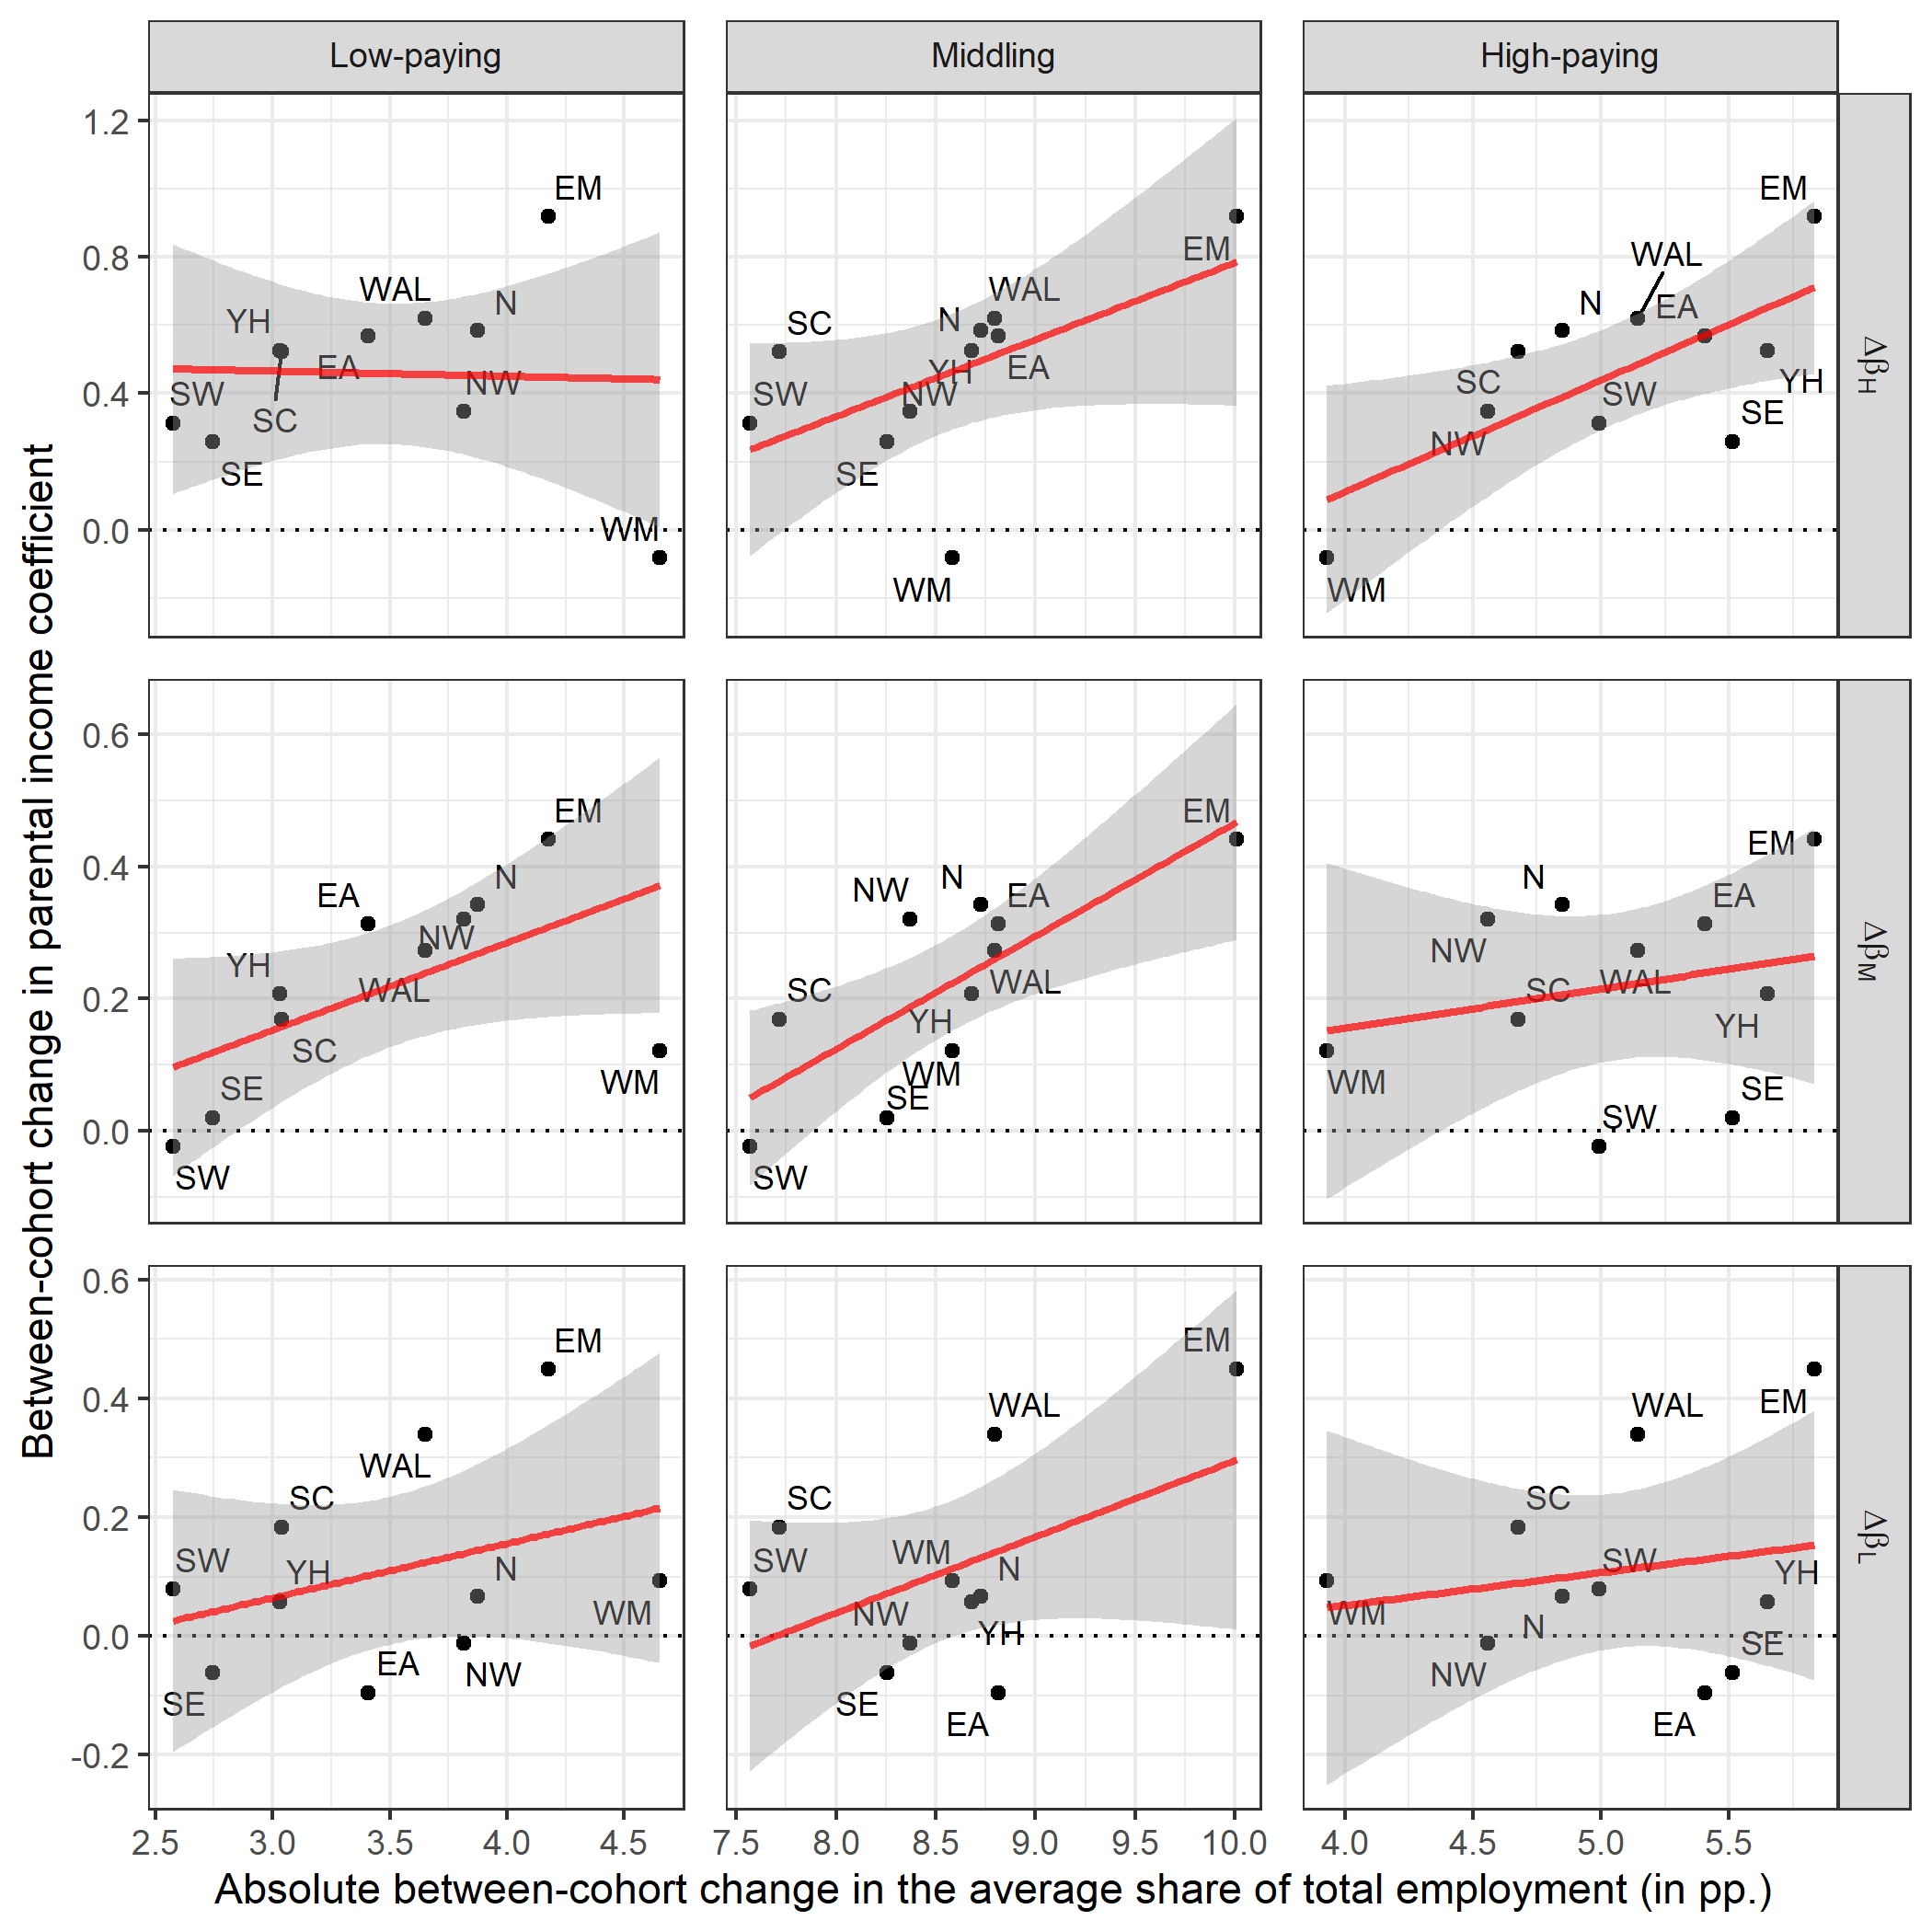
\includegraphics[width=\linewidth]{chap2/graphic/regocc-absolute-all.png}
    \vspace{-3em}
	\justify\singlespacing\footnotesize{\textit{Notes:} This figure presents the correlation across regions between the change in the parental income coefficient for each occupation (low-paying, middling, and high-paying) in second period $\Delta\beta_k$ and the between-cohort change in absolute value in the average share of total employment of low-paying, middling, and high-paying occupations, in percentage points. Note that, by taking the absolute value of the change, we reversed the x-axis for the middling panels (middle column). Thus, regions on the left-hand (resp. right-hand) side of each panel are those where the polarization of employment has been lower (resp. larger).}
\end{figure}